%\documentclass[../main/6103-LecturesNotes.tex]{subfiles}
%\begin{document}

\chapter{Differentiation}
\section{Rates of change}

Suppose we drive from UCL to Stratford-upon-Avon ($100$ miles). We plot a graph of the distance travelled against time. We want to measure how fast we traveled. The average speed of the trip is calculated as follows:
\begin{equation*}
\frac{100\text{ miles}}{2 \text{ hrs}}=50\text{ mph}.
\end{equation*}

\begin{figure}[H]
\centering
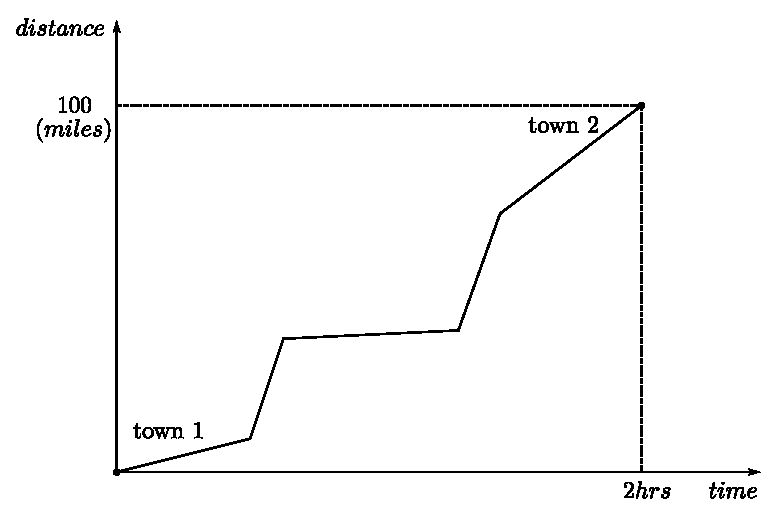
\includegraphics[scale=0.75]{img/distance-time-graph}
\caption{Graph showing distance travelled against time, from town 1 (UCL) to town 2 (Stratford-upon-Avon).}
\label{fig:distance-time-graph}
\end{figure}

However, when travelling you do not stick to one speed, sometimes you do more than $50$ mph, sometimes much less. The reading on your speedometer is your {\it instantaneous} speed. This corresponds to the {\it gradient} of the graph at the given point in your journey.

\begin{definition}
The \textbf{gradient} of a line is a measure of the steepness or slope of the line. It can be found using:
$$\text{gradient}=\frac{\text{change in }y}{\text{change in }x}$$

The gradient of a curve is the gradient of the tangent at a given point.
\begin{figure}[H]
\centering
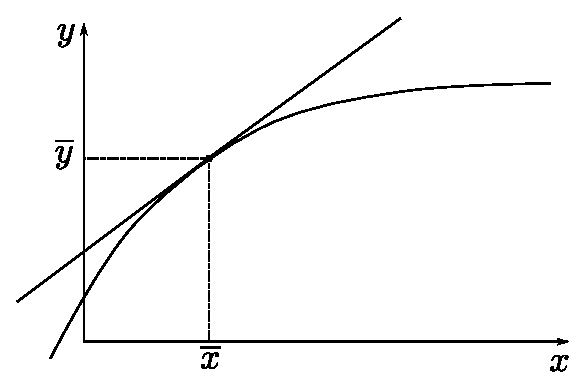
\includegraphics[scale=0.8]{img/tangent-line}
\caption{Curve $y=f(x)$ with tangent line at $(\overline{x},\overline{y})$.}
\label{fig:tangent-line}
\end{figure}

\end{definition}

In the following section, we will be looking at methods for finding the gradients of graphs.

\section{Finding the gradient}

For mathematical curves, we will learn to find gradients algebraically.

To find the gradient of a curve $y=q(x)$ at $x=c$, we first consider the line joining the points $(c,q(c))$ $(c+h,q(c+h))$, where $h$ is small.

\begin{figure}[H]
\centering
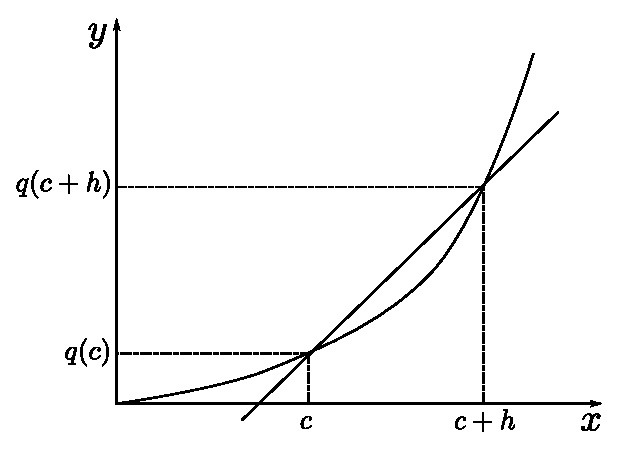
\includegraphics[scale=0.8]{img/chord}
\caption{Graph showing line joining the points $(c,q(c))$ and $(c+h,q(c+h))$ on the curve $y=q(x)$.}
\label{fig:chord}
\end{figure}

We will look at the gradient of this line as we make $h$ smaller and smaller, as this will get closer and closer to the gradient of the tangent.

\begin{example} 
Let us start with the example of the curve $y=S(x)=x^2$.

\begin{figure}[H]
\centering
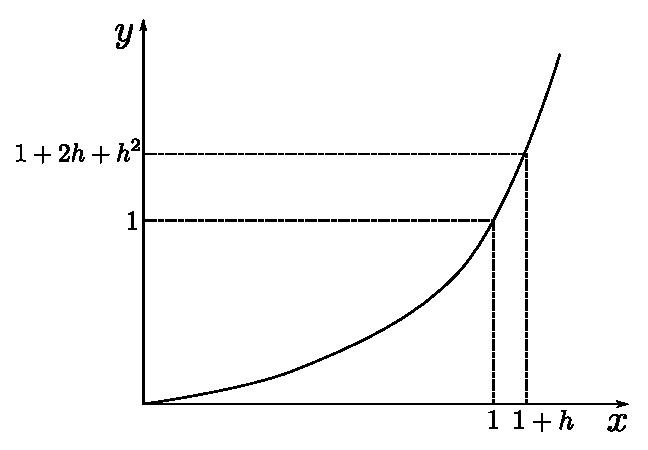
\includegraphics[scale=0.8]{img/increment-quadratic}
\caption{Curve $y=S(x)=x^2$ displaying small increment at $x=1$.}
\label{fig:increment-quadratic}
\end{figure}


Look at the point $(1,1)$ on the curve. We want find the gradient at this point. Lets consider a line connecting $(1,1)$ and $(1+h,(1+h)^2)$.

The gradient of this line is:

\begin{align}
\frac{\text{change in }y}{\text{change in }x} &= \frac{(1+h)^2-1}{1+h-1}\\
&=\frac{h^2+2h}{h}\\
&=h+2
\end{align}

To find the gradient at the point, we look at what will happen as $h\rightarrow0$ ($h$ tends to 0).

$$\text{As }h\rightarrow0\quad h+2\rightarrow2$$

Therefore the gradient of the curve $y=x^2$ at the point $x=1$ is $1$.

\end{example}

We define the derivative as follows:
\begin{definition}
The \textbf{gradient} of $y=f(x)$ at x=c, written $\frac{dy}{dx}\text{ at }c$ or $f'(c)$, is
$$f'(c)=\lim_{h\rightarrow 0}\frac{f(c+h)-f(c)}{h}.$$
\end{definition}

$\lim_{h\rightarrow0}$ is the limit as $h$ gets closer and closer to 0. This definition is exactly what we used in the example.

If we leave $c$ as a variable instead of subsituting in a value, we can find the gradient of the whole curve.

\begin{example}\label{cubic-ex-deriv}
Let us consider the function $q(x)=x^3$. At $x=c+h$ we have
\[q(c+h)=(c+h)^3=c^3+3c^2h+3ch^2+h^3.\]
Therefore,
\begin{align}
q'(c)&=\lim_{h\rightarrow0}\frac{c^3+3c^2h+3ch^2+h^3-c^3}{h}\\
&=\lim_{h\rightarrow0}\frac{3c^2h+3ch^2+h^3}{h}\\
&=\lim_{h\rightarrow0}3c^2+3ch+h^2\\
&=3c^2
\end{align}
or in other words, \[q'(x)=3x^2.\]
\end{example}

\begin{example}
Now let us consider the function $r(x)=1/x$. In this case we have
\[r(c+h)-r(c)=\frac{1}{c+h}-\frac{1}{c}.\]
Now, let us consider the ratio
\[\frac{r(c+h)-r(c)}{h}=\frac{1}{h}\left(\frac{1}{c+h}-\frac{1}{c}\right)=\frac{1}{h}\left(\frac{-h}{c(c+h)}\right)=-\frac{1}{c(c+h)},\]
and as $h\to0$, we have
\[r'(c)=-\frac{1}{c^2},\quad \text{i.e.}\quad r'(x)=-\frac{1}{x^2},\quad x\ne0.\]
\note{$r(x)=1/x$ is not well defined at $x=0$ and in this case, nor is its derivative.}
\end{example}

%\end{document}
